% Appendix A

\chapter{Google Test} % Main appendix title

\label{AppendixC} % For referencing this appendix elsewhere, use 

In this appendix, Google Test is explained in more detail, along with some examples and how it has been applied to this application.

\section{Google Test}
Google Test, or Google C++ Testing Framework, is a tool developed by Google. As a Testing Framework, it allows the definition of functions called \emph{TEST()} which do two things:
\begin{itemize}
	\item Executes some functionality of the code
	\item Compares the output with the expected output to detect unexpected and erroneous behaviour.
\end{itemize}

Let us evaluate the following test:
\begin{verbatim}
TEST(FactorialTest, Positive) {
    EXPECT_EQ(1, Factorial(1));
    EXPECT_EQ(2, Factorial(2));
    EXPECT_EQ(6, Factorial(3));
    EXPECT_EQ(40320, Factorial(8));
}
\end{verbatim}
FactorialTest is the test case name which is used for defining test groups. For example, if the programmer wanted to test Factorial behaviour for negative input, he/she could have difined \emph{TEST(FactorialTest,Negative)}. Positive is the test name.\\
As the reader can see, what the test is doing is checking that the output of the function is equal to the expected output. \emph{EXPECT\_EQ(1,Factorial(1));}

\section{Google Test for this project}
All the tests done for this project can be found inside the \emph{test\_files} folder.\\
The folder contains three types of files:
\begin{itemize}
	\item *\_UT.cpp : Unit Tests
	\item *\_INT.cpp : Integration Tests
	\item *\_Stup.cpp : Stub class
\end{itemize}
Unit testing is a software testing where individual units/components of the software are tested. Its purpose is to validate that each component works as expected. The majority of tests done for this project are Unit Tests. The first reason is that of the methodology which has been Test Driven Development. The second reason is that Unit Tests are more straightforward to generate and they reveal unexpected beahviour closer to the source.\\
An example of UT in this project could be \emph{PBMin\_UT.cpp}:
\begin{verbatim}
TEST(GetFirstFreshVariable,getFirstFreshVariable){
	std::vector< PBConstraint > e_constraints = {
		PBConstraint(PBFormula({1,2},{1,2}),1),
		PBConstraint(PBFormula({3,4},{2,3}),1),
		PBConstraint(PBFormula({3,7},{1,3}),1)
	};
	PBMin m = PBMin(e_constraints, PBFormula({3,-5},{-1,2}));
	EXPECT_EQ(m.getFirstFreshVariable(), 4);
}
\end{verbatim}
For example, this test checks that the implementation of the function \emph{getFirstFreshVariable()} works as expected.\\
Integration testing is a software testing where individual units/components of software are combined and tested as a group. This type of testing has been used for testing the solvers with the search strategies which depend on them.\\
An example of INT in this project could be \emph{GeneralTimeoutSolver\_BinarySearchStrategy\_INT.cpp}:
\begin{verbatim}
TEST(Solve,problem3){
	std::vector< PBConstraint > constraints = {
		PBConstraint(PBFormula({2,2},{1,-1}),1),
		PBConstraint(PBFormula({3,4},{2,3}),1),
		PBConstraint(PBFormula({3,7},{1,3}),1)
	};
	PBFormula costFunction({-1,-3,7,-5},{1,-1,2,-2});
	bool e_sat = false;
	int64_t e_min = -8;
	std::vector< int32_t > e_model = {-1};
	BinarySearchStrategy bs;
	PBMin m = PBMin(constraints, costFunction);
	GeneralTimeoutSolver s(5,&bs,m);
	std::vector< int32_t > model;
	int64_t min;
	bool sat = s.run(model,min);
	EXPECT_EQ(sat, e_sat);
}
\end{verbatim}
This test how \emph{GeneralTimeoutSolver} and \emph{BinarySearchStrategy} work together.\\
Finally, a Stub class was done in order to test a component which relies on an unimplemented class at that time. In a nutshell, a Stub class is a class which simulates a behaviour. \\
An example of a Stub class in this project could be \emph{SlowSearchStrategy\_Stub.cpp}:
\begin{verbatim}
void loop(void (Solver::*solver)(std::vector< int32_t > &, const
std::vector< std::vector< int32_t > > &, bool &),std::vector< int32_t > &
model, int64_t & min, bool &sat, Solver *s, const PBMin &p) override {
	sleep(2);
	model.clear();
	model.push_back(1);
	model.push_back(2);
	model.push_back(3);
	min = 123;
	sat = true;
}
\end{verbatim}
This class calls the \emph{sleep(2)} function in order to test the implemented timeouts. As the reader can see, it is not a real implementation of a \emph{Solver} because its purpose is not to test itself but the timeouts.

\section{Google Test results}
Once a test file is compiled, it can be executed. Google Test framework will execute all the tests and do the required checks. The output is shown through the terminal.
\begin{center}
	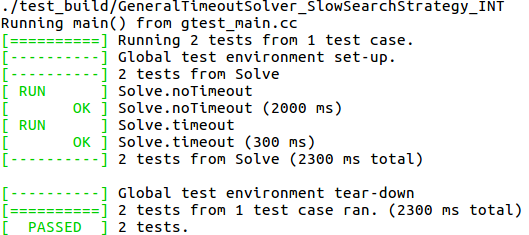
\includegraphics[width=0.9\textwidth]{Figures/google-test-output.png}
	\captionof{figure}{Google Test results from command line}
	\label{google-test-output}
\end{center}
The figure above\ref{google-test-output} was the output from \emph{GeneralTimeoutSolver\_SlowSearchStrategy\_INT} test suite. As the reader can see, the output from the test suite was the name of the test executed and if it passed the checks or not.  If a test does not pass the checks, the output becomes red, and the comparison which failed is printed. 